\section{Anhang}
\subsection{Abbildungen}
 \begin{figure}[htp]
  \begin{center}
   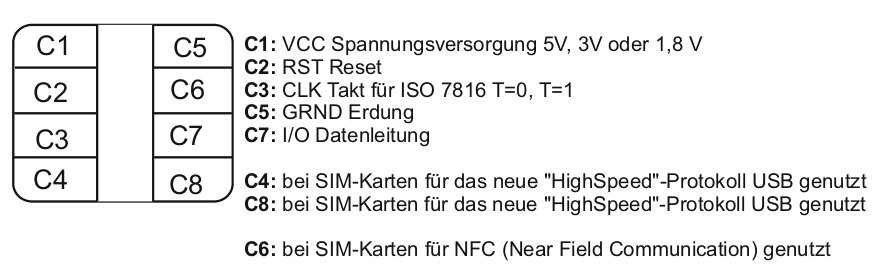
\includegraphics[width=410pt]{pinbelegung_chipkartensicherheit}
  \end{center}
  \caption[Pinbelegung einer Chipkarte]{Pinbelegung einer Chipkarte nach ISO/IEC 786 \cite{spitz11}}
  \label{abb:pinbelegung_chipkarten}
 \end{figure}

 \begin{figure}[htp]
  \begin{center}
   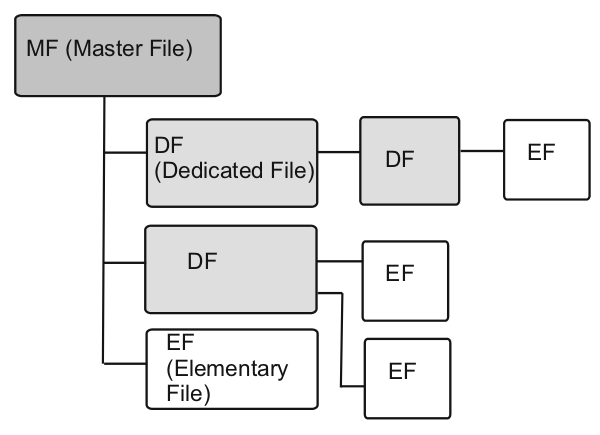
\includegraphics[width=350pt]{filesystem_chipkarten_chipkartensicherheit}
  \end{center}
  \caption[Filesystemarchitektur einer Chipkarte]{Filesystemarchitektur einer Chipkarte nach ISO/IEC 786 \cite{spitz11}}
  \label{abb:filesystem_chipkarten}
 \end{figure}

  \begin{figure}[htp]
  \begin{center}
   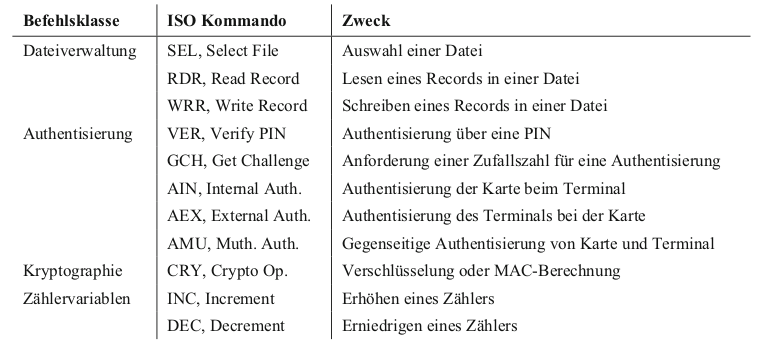
\includegraphics[width=460pt]{befehlsklassen_chipkartensicherheit}
  \end{center}
  \caption[Befehlsklassen einer Chipkarte]{Befehlsklassen einer Chipkarte nach ISO/IEC 786 \cite{spitz11}}
  \label{abb:befehlsklassen_chipkarten}
 \end{figure}

  \begin{figure}[htp]
  \begin{center}
   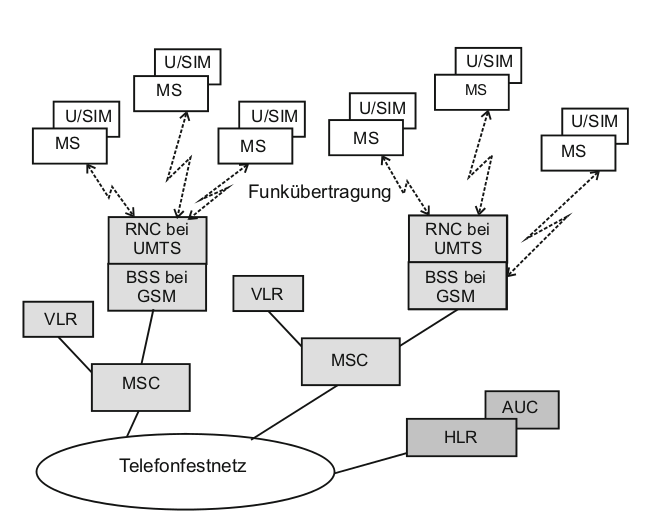
\includegraphics[width=380pt]{teilnehmer_telefonnetz_chipkartensicherheit}
  \end{center}
  \caption[Teilnehmer in Mobilfunknetzen]{Teilnehmer in Mobilfunknetzen (GSM und UMTS) \cite{spitz11}}
  \label{abb:teilnehmer_telefonnetz}
 \end{figure}

  \begin{figure}[htp]
  \begin{center}
   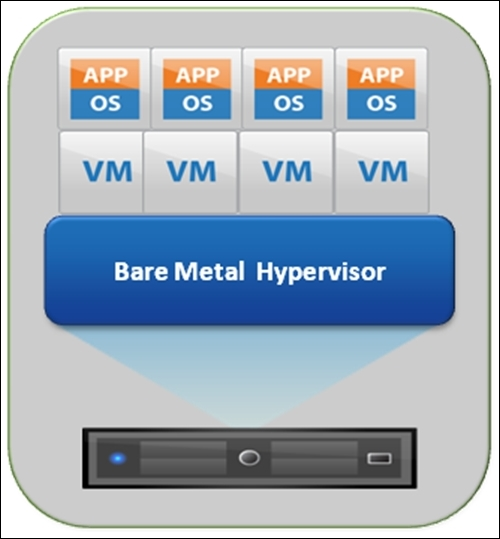
\includegraphics[width=200pt]{hypervisor_type1_dash13}
  \end{center}
  \caption[Architektur eines Typ-1-Hypervisors]{Architektur eines Typ-1-Hypervisors \cite{dash13}}
  \label{abb:hypervisor_type1}
 \end{figure}

  \begin{figure}[htp]
  \begin{center}
   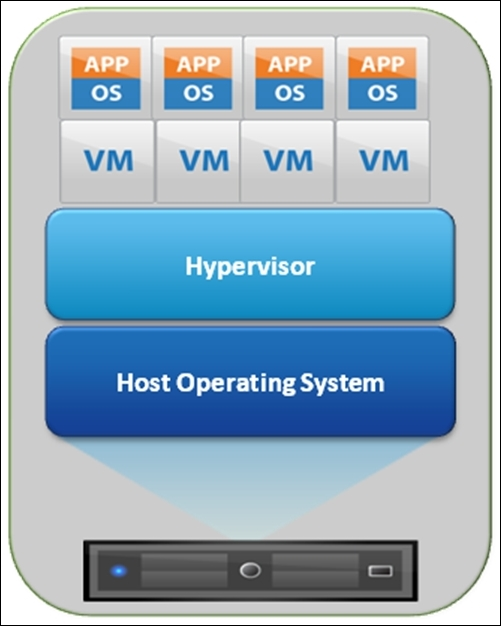
\includegraphics[width=200pt]{hypervisor_type2_dash13}
  \end{center}
  \caption[Architektur eines Typ-2-Hypervisors]{Architektur eines Typ-2-Hypervisors \cite{dash13}}
  \label{abb:hypervisor_type2}
 \end{figure}

  \begin{figure}[htp]
  \begin{center}
   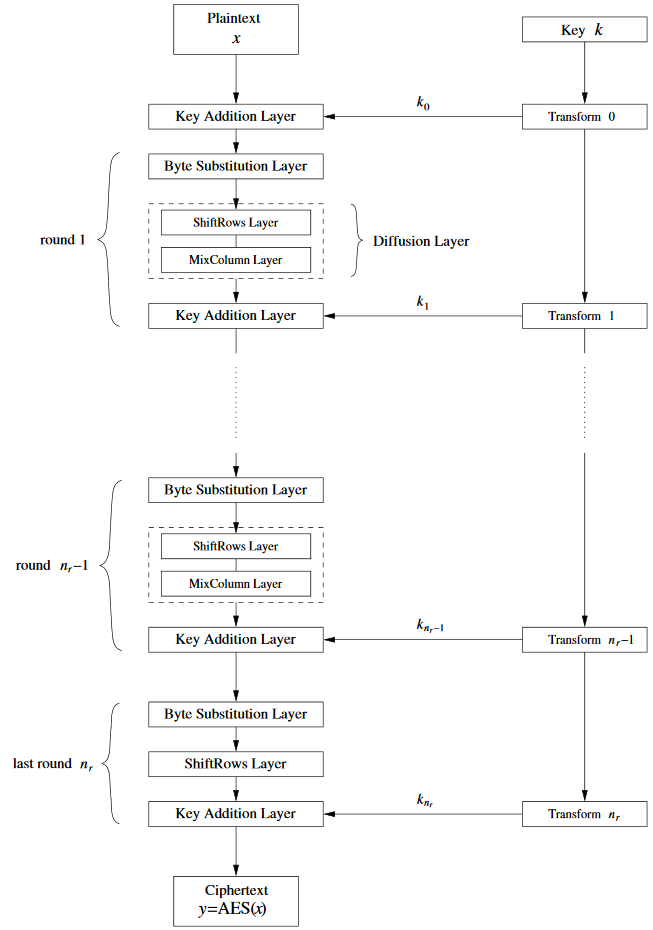
\includegraphics[width=440pt]{ablauf_aes}
  \end{center}
  \caption[Grafische Darstellung der AES-Verschlüsselung]{Grafische Darstellung der AES-Verschlüsselung \cite{paar10}}
  \label{abb:funktion_aes}
 \end{figure}
 
  \begin{figure}[htp]
  \begin{center}
   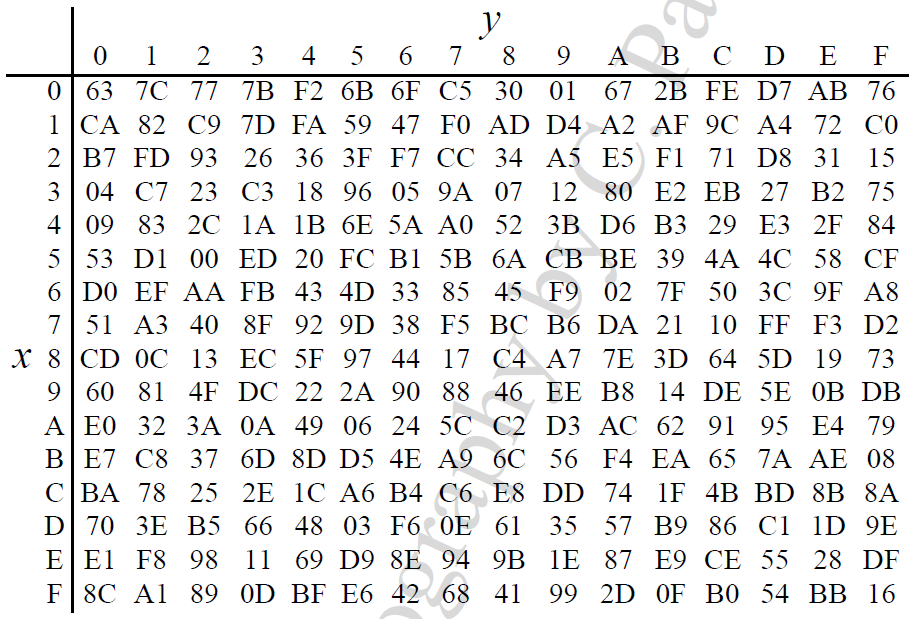
\includegraphics[width=440pt]{s-box}
  \end{center}
  \caption[Substitutionstabelle für AES-Verschlüsselung]{Substitutionstabelle für AES-Verschlüsselung \cite{paar10}}
  \label{abb:s-box}
 \end{figure}
 
 \begin{figure}[htp]
  \begin{center}
   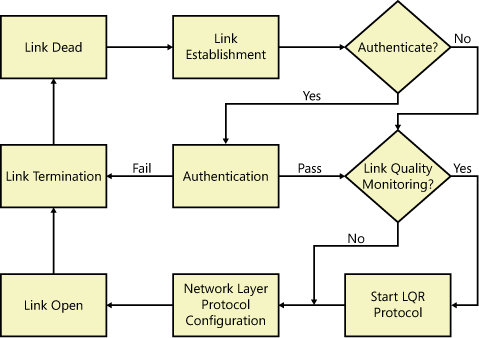
\includegraphics[width=350pt]{aufbauphasen_pppverbindung}
  \end{center}
  \caption[Aufbauphasen einer PPP-Verbindung]{Aufbauphasen einer PPP-Verbindung \cite{zackercomptia}}
  \label{abb:aufbauphasen_pppverbindung}
 \end{figure}

 \begin{figure}[htp]
  \begin{center}
   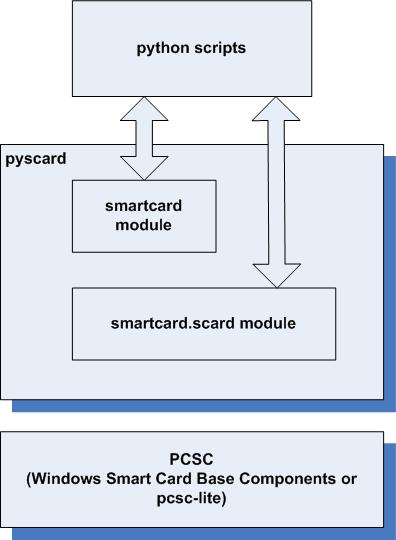
\includegraphics[width=350pt]{pyscard_schema}
  \end{center}
  \caption[Architektur der pyscard-Bibliothek]{Architektur der pyscard-Bibliothek \cite{pyscardweb}}
  \label{abb:pyscard_schema}
 \end{figure}

 \clearpage

\subsection{Listings}

  \lstinputlisting[caption=main.c, language=c, label=lst:main.c]{main.c}

  \lstinputlisting[caption=milenage.c, label=lst:milenage.c]{milenage.c}

  \lstinputlisting[caption=rijndael.c, language=c, label=lst:rijndael.c]{rijndael.c}

  \lstinputlisting[caption=client.py, language=python, label=lst:client.py]{client.py}

  \lstinputlisting[caption=..ppp/pppoe.conf, label=lst:pppoe.conf]{pppoe_conf}
 
% \lstinputlisting[caption=...ppp/allip, label=lst:allip]{allip}

 \lstinputlisting[caption=...ppp/pppoe-server-options, label=lst:pppoe_server_options]{pppoe-server-options}

 \lstinputlisting[caption=...init.d/pppoed, language=bash, label=lst:pppoe_init]{pppoed_init}
